% Latex Style for CMP PGR DAY 2009.
%
% Revision 1.0
% Feb. 12 2009.
%
% Barry-John Theobald, University of East Anglia, Norwich, UK

\documentclass{cmppgr}

\usepackage[pdftex]{graphicx}
\graphicspath{{figures/}}

\input{t1pcr.fd}
\makeatother
\setlength{\footnotesep}{3ex}
\usepackage{listings}
\usepackage{pgfplots}
\usepackage{subcaption}
\usepackage{subcaption,siunitx,booktabs}

\title{Probabilistic approach over Decision Trees for problems with discrete data, medium number of instances and a small to medium number of attributes 2017 --- Norwich, UK}
\name{Luke M. Garrigan}
\institution{
	Machine Learning, University of East Anglia, UK
}
\email{l.garrigan@uea.ac.uk}



\begin{document}
\maketitle

\begin{abstract}

Bayesian classifiers are widely known for their optimality when attributes are independent given the class. This paper attempts to prove that small samples of discrete data with arbitrary dependencies are more accurately classified using a probabilistic approach over decision trees. 


\end{abstract}

\keywords{Probabilistic, Naive Bayes, Decision Trees}

\section{Introduction}

In machine learning a learner algorithm is given a set of training instances with their corresponding class labels, it then produces a classifier. The classifier takes unlabelled testing instances and assigns it to a class. Choosing the best suited algorithm specific to the sample set is not a trivial process.

Probabilistic classification is the application of approximating a joint distribution with a product distribution. Bayes rule is used to approximate the conditional probability of a given class label. Approaches such as \textit{naive} Bayes are among the most popular classifiers used in the machine learning community. Derived from generative probability models they are generally easy to understand and the induction of these classifiers is extremely fast, requiring only a single pass through the data if all attributes are discrete \cite{kohavi1996scaling}. The \textit{naive} Bayes classifier is the simplest of models in this paper, it assumes that all attributes are independent of each other given the context of the class. Although the \textit{naive} assumption of independence is not true in terms of most sample sets, many papers such as \cite{domingos1997optimality} have proven that \textit{naive} Bayes classification accuracy is very competitive when compared with more complex state-of-the-art algorithms. 

 

Decision trees classify instances by sorting them down the tree from the root to some leaf node which represents the classification of the given instance. Nodes specify a test of some attribute of the instance and each branch from that node corresponds to one of the possible values for this attribute. A given instance is classified moving down the tree, the attribute specific to that node is tested. Following down the branch corresponding to the value of the attribute in the given example, this is then repeated until a leaf node is reached and a classification is made. Decision trees are convenient due to their transparency, they explicitly display all possible alternatives and pursues these alternatives to a conclusion. This allows for a comprehensive analysis of the consequences of each decision.

 


\section{Data Description}
\begin{itemize}
	\item \textit{Teaching Assistant} consists of evaluations of teaching performance the scores are divided into 3 roughly equal-size categories ("low", "medium," and "high").
	\item \textit{Seeds} comprises of data belonging to three different varieties of wheat: Kama, Rosa and Canadian. The classification is to determine which wheat it is given its characteristics
	\item \textit{Breast Cancer} is data to determine whether a tumor has the ability to invade neighbouring tissue. (Benign or Malignant) 
	
    \item \textit{Ecoli} 
	\item \textit{Glass} classification of types of glass, motivated by criminology investigation.
	\item \textit{Haberman} is data from the survival of patients who had undergone surgery for breast cancer.
	\item \textit{Hayes Roth}
	\item \textit{Heart}
	\item \textit{Lymphography} provided by the Oncology Institute to determine whether tumours are metastases, malign or fibrous.
	\item \textit{Promoters} is data for promoter gene sequences (DNA), the class labels are binary, either a promoter or not a promoter.
	\item \textit{Shuttle Landing} rules for determining the conditions under which an autolanding would be preferable to manual control of the spacecraft the class label is either auto or noauto.
	\item \textit{Sonar} patterns obtained by bouncing sonar signals off a metal cylinder at various angles and under various conditions. The label associated with each record contains the letter "R" if the object is a rock and "M" if it is a mine (metal cylinder).
	\item \textit{Thyroid}
	
\end{itemize}

\subsection{Case Study}
\subsubsection{Dataset Information}
Electroencephalography is a domain concerning recording and interpretation of the electroencephalogram (EEG). EEG is a record of the electric signal generated by the cooperative action of brain cells, or more precisely, the time course of extracellular field potentials generated by their synchronous action\cite{lindsley1950emotions}. EEG detects electrical activity in the brain using small, flat metal discs (electrodes) attached to the scalp. An EEG is used for diagnosing brain disorders, most frequently epilepsy. 



For the current study, EEG data was collected 5 times on various days from a healthy right-handed subject of 25 years of age. The data was recorded on a Medelec Profile Digital EEG machine. The settings of high-frequency filter 50 Hz, low frequency filter 1.6 Hz, notch filter 50 Hz, sensitivity 70 micro volts/mm, and a sampling rate of 256 Hz were used for the basic signal processing. 

In summary, the subject was asked to lie down in a relaxed position with eyes closed. The EEG recorded for the relaxed state for 5 minutes.Following this, an audible beep of 60 dB for 0.91 seconds was given before and after the subject was asked to mentally plan lifting of the right-hand thumb (no actual movement), after a gap of 5 minutes the same cue is given to repeat the experiment lasting approximately 30 minutes \cite{planning_relax_data_set}.

\subsubsection{Attribute Information}
By applying wavelet packet analysis on the original signal 12 wavelet coefficients in the 7-13 Hz frequency band were obtained. This is a classification problem to determine whether the subject is relaxing or planning. There are 182 instances; the univariate dataset contains 12 real attributes and a binary class label.
 









\begin{table}[h]
	\centering
	\caption{Details of the data used. C=Categorical, I=Integer, R=Real}
	\begin{tabular}{|l|c|c|c|c|}
		\hline
		Dataset & Inst/Attr& Attr Type &Class \# \\\hline\hline
		Teaching Assistant & 151/5& C,I & 3 \\
		Seeds & 210/7& R & 3 \\
		Planning Relax & 182/13&R & 2 \\
		Breast Cancer & 286/9& C & 2 \\
		Ecoli & 223/10 & R & 8 \\
		Glass & 141/6  & R& 2 \\
		Haberman & 203/4 &R & 2 \\
		Hayes Roth & 160/5 & C & 3 \\
		Heart & 169/14& R& 2 \\
		Lymphography & 148/18 & C& 4 \\
		Promoters & 106/58  &C & 2 \\
		Shuttle Landing & 252/7 &C& 2 \\
		Sonar & 137/60&R & 2  \\
		Thyroid & 142/6& R & 2 \\\hline
	\end{tabular}
	\label{tab:example}
\end{table}




\section{Classifier Description}
\subsection{Probabalistic}
\subsubsection{\textit{Naive} Bayes}
\textit{Naive} Bayes was selected for testing due to its popularity for classification problems and its presence in the machine learning community. As its name suggests its assumptions are naive and are not generally concordant with the data; it assumes all attributes are independent of each other given the context of the class but has been shown to perform surprisingly well in many classification problems. It is computationally efficient as training is linear in both the number of instances and attributes \cite{frank2002locally}. 

Let $C$ represent the classification variable, and let $C_k$ be the value of $C$.
According to Bayes Rule, the probability of an instance $X$ with attributes $X = (x_1, x_2,.. , x_n)$
having class label $C_k$ is
$$ P(C_k \mid X) = \frac{P(X \mid C_k) \, P(C_k)}{P(X)} $$
where $P(C_k \mid X)$ represents the posterior probability of class c given a predictor $X$. $P(X\mid C_k)$ is the likelihood; the probability of the predictor given $C_k$. $P(C_k)$ is the prior probability of $C_k$; the current knowledge of the class distribution and $P(X)$ is the predictor prior probability.

\textit{naive} Bayes assumes that all attributes are independent given the value of the class label.

$$P(X|C_k)=P(x_1, x_2,.. , x_n \mid C_k) = \prod_{i=1}^{n}P(x_i|C_k) $$

So the conditional distribution over the class variable $C$ can be represented by:
$$P(C_k \mid x_1,.. x_n) = \frac{1}{Z}P(C_k)\prod_{i=1}^{n}P(x_i \mid C_k)$$
where $Z$ is a scaling factor dependent on $x_1, x_2,.. , x_n $. In order to build a classifier from this, a decision rule is used by picking the classification which is most probable; for two posterior probabilities $P(C_1|X)= 0.54$ and $P(C_2|X) =0.46$ using the \textit{maximum a posteriori} (MAP) rule, the larger of the two is chosen \cite{zhang2004optimality}.


\subsubsection{Bayesian Networks}
Bayesian networks belong to the family of probabilistic graphical models. Graphical model expresses the conditional dependence structure between random variables and are used to represent knowledge about uncertain domains. Nodes within a Bayesian network represent the random variables, edges represent the conditional dependencies; nodes not connected are conditionally independent of each other. Each node is associated with a probability function that takes as input a particular set of values for the node's parent variables and outputs the probability of the variable represented by the node \cite{heckerman1995learning}.

In Bayesian networks each node is conditionally independent of any subset of nodes that are not descendants of itself gives its parent, so the value of a node is conditional only on the values of its parent nodes. Let $V$ represent a node in the graph and $par(V_i)$ be the parent of the node:
$$P(V_1, V_2, \dots V_n) = \prod_{i=1}^{n}P(V_i \mid par(V_i))$$

So to compute the joint probabilities we must calculate the conditional probability between itself and its parent for each node in the graph. The chain rule is then computer to determine the graphs joint probability functions. 

$$P(V_1, V_2, \dots V_n) = P(V_1)P(V_2 \mid V_1)P(V_3 \mid V_1, V_2)$$


\textit{Prior probabilities} are nodes without parents; they are not conditioned on other random variables \cite{jensen1996introduction}.


Bayesian networks do not necessarily imply a commitment to Bayesian statistics, it is common to use frequentists methods to estimate the parameters of the CPDS.


\subsection{Decision Trees}
\subsubsection{C4.5}
C4.5 is an algorithm used to build decision trees, they are created using a divide-and-conquer approach. The tree is formed using information entropy as found in the ID3 algorithm which is a precursor to C4.5, however, this paper only covers the C4.5 algorithm. C4.5 offers a number of improvements over ID3: handling data with missing values, accepts both continuous and discrete attributes, handling attributes with different costs and solves over-fitting by pruning. Ross Quinlan's latest iteration is the C5.0 algorithm which he states is several orders of magnitude faster than C4.5 \cite{quinlan2004data}, unfortunately, this software is proprietary thus not compared.

Entropy is a measure of unpredictability, Shannon entropy calculates the level of uncertainty:
$$Entropy(P) = -\sum_{i=1}^{n}P_i(\log_2P_i)$$

Information gain measures the expected reduction in entropy caused by partitioning according to the given attribute.
$$Gain(S,A)=Entropy(S)- \sum_{v in Values}^{}\frac{|S_v|}{|S|}Entropy(S)$$

C4.5 is implemented recursively, let $T$ be the set of training instances, the algorithm chooses an attribute that best differentiates the instances contained in $T$, a tree node is created with the value of the chosen attribute. Child nodes are created each link represents a unique value for the given attribute, the child values are then used to further subdivide the instances into subclasses. The subclasses either satisfy the predefined criteria or the remaining attributes choice for the path is null, this is repeated recursively. The classifications for the testing instances is made by following the decision path.

\subsubsection{Random Forests}
Meta-algorithms are approaches to combine several machine learning techniques into one predictive model in order to decrease the variance (bagging) or bias (boosting) \cite{galkin}. 


Ensemble learning methods generate many classifiers and aggregate their results. Random forest incorporates a supplementary layer of randomness to bagging, in addition to constructing each tree using a different bootstrap sample of the data.
Random forests construct the classification distinctly using the best among a subset of predictors randomly chosen at that node \cite{liaw2002classification}. Although the approach is somewhat counter-intuitive it has been shown to outperform many state-of-the-art classifiers.


\subsubsection{Logistic Model Trees}
Logistic Model Trees (LMT) use a combination of a tree structure and logistic regression models to for a single tree. \cite{landwehr2005logistic} performed experiments showing that LMT produces more accurate classifiers than C4.5, CART, logistic regression, model trees, functional trees, \textit{naive} Bayes trees and Lots.


LMT is a combination of learners which rely on logistic regression models.
Logistic regression is used to describe data and to explain the relationship between one dependent binary variable and one or more nominal, ordinal, interval or ratio-level independent variables \cite{statistics_solutions}. LMT uses cost-complexity pruning. The compute time of LMT is much greater than the other algorithms.

\section{Preliminaries}
\subsection{Discretization}
Discretization concerns with the process of transferring continuous data into discrete counterparts. Numeric attributes were discretized into ten equal-length intervals unless the number of uniquely observed values for an attribute was less than 10. This approach was compared in \cite{dougherty1995supervised} with entropy-based and purity-based methods, which are supervised algorithms. An empirical evaluation showed that the \textit{naive} Bayes algorithm significantly improved accuracy when features were discretized using an entropy-based method. However, due to its simplicity, the unsupervised binning discretization method was used for all continuous attributes.
\subsection{Methods For Accuracy Estimation}







\subsubsection{K-Fold Cross-Validation}
Cross-validation is a computationally expensive algorithm used to estimate performance, it uses all available instances as both training and testing sets. The dataset is split into $k$ equally sized non-overlapping subsets $S$. Given a fold $S_i$ a model is trained on $S \setminus S_i$, then $S_i$ is used to create the accuracy estimation.

\subsubsection{Leave-One-Out Cross-Validation (LOOCV)}
Leave-One-Out Cross-Validation is  K-fold cross validation where $K$ is equal to the number of instances in the dataset. The classifier is trained on all data except the one instance being left, this is repeated until all instances in the dataset have been the test instance. An average of the data is collected and used to evaluate the classifier.

\subsubsection{Bias And Variance Tradeoff}
As $k$ increases the less bias the classification is in overestimating the true expected error as the folds will be closer to the total dataset. However, in doing this it induces variance. To minimise the testing bias a large portion of the dataset must be used for training, meaning not much data is used for testing, this ensures that the model will be as close as possible to the model achievable by training using the entire dataset. Minimising the testing variance would mean quite the opposite, a large amount of data would be used for testing, this ensures a more reliable estimate error of the classifier.

\begin{figure}[!ht]
	\begin{subfigure}[b]{0.40\textwidth}
		\begin{tikzpicture}
		\begin{axis}[
		width=\textwidth,
		xlabel = Folds,
		ylabel = Percent Accuracy,
		xtick=data,
		xticklabels={2,5,10,20,30,-5,-2,-1},
		]
		\addplot[mark=square,error bars/.cd, y dir=both, y explicit, ] coordinates{
			(1,78.25891)+=(0,1.27109)-=(0,1.26891)
			(2,81.65178)+=(0,0.7822)-=(0,0.80178)
			(3,81.83036)-=(0,0.60036)+=(0,0.59964)
			(4,82.5)-=(0,0.56)+=(0,0.56)
			(5,82.45537)-=(0,0.365)+=(0,0.374)
			(6,82.1429)
			(7,82.1429)
			(8,82.1429)};
		
		
		\legend{Ecoli}
		\end{axis}
		\end{tikzpicture}
	\end{subfigure}
	\caption{Bias representation of cross-validation. The negative k-folds shows leave-k-out, -1 is LOOCV.}
\end{figure} 

Figure 1 shows the bias and variance of k-fold cross-validation on arbitrary datasets using \textit{naive} bayes. More in-depth experiments have been conducted and state that for real-world data the best method for cross-validation is ten-fold stratified and that even if you have the computational power to use more folds ten-fold is the better option \cite{kohavi1995study}. Ten-fold stratified cross-validation was used for experiments in this paper. 
 
 
\subsection{Missing Values}
For scenarios such as $P(X_1=x_1 \dots X_k=? \dots X_n=x_n|c)$ where $?$ represents a missing value, \textit{naive} Bayes skips over the missing value:
$P(x_1 \dots X_k \dots x_n \mid c)= \prod_{i \neq k }^{n}P(x_i \mid c)$.  The documentation of J48 implementation of C4.5 states that any split on an attribute with missing value will be done with weights proportional to frequencies of the observed non-missing values \cite{witten2016data}. In this paper missing values were ignored completely, in an attempt to ensure that certain models don't have an advantage over others.
 
\subsection{Zero Counts}
Zero counts are when a class value and attribute value have never occurred together in the training set; this doesn't necessarily mean that this data is never going to be apart of a testing set. Laplace correction was used as a fail safe. Let $N_{ijk}$ represent the number of examples where $X_i=x_k$ and $C=C_j$, let $N_j$ represent the number of instances of class $c_j$ and $k$ the number of possible values of $Xi$. When computing the conditional probabilities rather than using the estimate $P(X_i= x_k | c_j) =\frac{N_{ijk}}{N_j}$, Laplace correction was used:

$$P(X_i = x_k \mid C_j)= \frac{N_{ijk}+1}{N_j+k}$$
 

\section{Results}

\begin{table*}[t]
	\centering
	\caption{Classification accuracies and sample standard deviation, using 20 iterations of ten-fold cross-validation.}
	\begin{tabular}{|l|c|c|c|c|c|c|}
	\hline
Dataset & \textit{Naive} Bayes & Bayes Net & C4.5 &Random Forests & LMT \\\hline\hline
Teaching Assistant &  54.01$\pm$11.02 &   46.32$\pm$7.74 &  57.41$\pm$12.64 &    67.54$\pm$11.35 &  53.27$\pm$11.08  \\
Seeds & 89.38$\pm$7.09 & 89.76$\pm$7.05  &   89.57$\pm$7.09    & 89.81$\pm$6.42  &   90.38$\pm$6.35 \\
Planning Relax & 56.59$\pm$9.41 &   55.23$\pm$9.72  &   71.46$\pm$1.53 &  71.72$\pm$4.61 &   71.02$\pm$3.15\\
Breast Cancer & 72.88$\pm$8.61 &   72.69$\pm$8.87   &  76.11$\pm$5.44  &   73.51$\pm$7.34&    74.31$\pm$6.69\\
Ecoli &  81.88$\pm$7.28 &    83.22$\pm$6.64  &    71.65$\pm$6.90 &    76.52$\pm$6.66 &    81.30$\pm$8.08 \\
Glass & 93.98$\pm$6.50 &   94.98$\pm$6.48  &   85.00$\pm$7.91 &   92.44$\pm$7.30 &    89.07$\pm$9.04\\
Haberman &  73.54$\pm$6.90 &    73.48$\pm$7.09  &    73.12$\pm$2.90 &     67.82$\pm$8.97 &     72.17$\pm$6.43\\
Hayes Roth &83.83$\pm$8.01 &   83.96$\pm$7.97   &  72.27$\pm$8.46 &   80.90$\pm$9.33   &  85.15$\pm$7.79\\
Heart &  81.17$\pm$8.16  &  81.17$\pm$7.57    &  75.06$\pm$9.69    &  77.94$\pm$9.62   &   80.28$\pm$8.30\\
Lymphography & 84.04$\pm$9.43  &    85.46$\pm$8.78   &    79.12$\pm$9.96  &     83.33$\pm$9.84   &    81.86$\pm$9.82  \\
Promoters & 91.14$\pm$8.71  &  91.14$\pm$9.12   &   77.45$\pm$12.79  &   91.05$\pm$9.37    &  90.41$\pm$9.15\\
Shuttle Landing & 93.26$\pm$4.56 &   93.26$\pm$4.56   &   96.59$\pm$3.63   &   98.30$\pm$2.64 &    98.41$\pm$2.52 \\
Sonar & 73.49$\pm$9.68 &   73.27$\pm$9.85  &    62.90$\pm$11.07  &   74.85$\pm$11.17   &   72.09$\pm$11.81  \\
Thyroid & 91.32$\pm$6.49 &  92.87$\pm$6.40   &   90.13$\pm$7.13    &  91.88$\pm$6.18   &   90.56$\pm$7.18 \\\hline
Mean &   80.04 &  79.77    &   76.99    &   81.26    &     80.73  \\\hline
	\end{tabular}
	\label{tab:example}
\end{table*}

Table 2 displays the average classification accuracies and sample standard deviations over 20 iterations of ten-fold cross-validation. All 14 data-sets were classified using each algorithm.

Planning Relax was specifically chosen as a case study as it goes against the initial hypothesis and rather significantly; all decision tree algorithms output higher classification accuracies than both probability algorithmsF for this dataset. This could be for a number of reasons, 
it is possible that some of these datasets contain little attribute dependencies, this could result in \textit{naive} Bayesoutperform the other or on the contrary the attributes could have significant dependencies meaning \textit{naive} Bayes would likely perform poorly. To come to any conclusion a measurement of attribute dependence must be carried out.


\subsection{Timing Experiment}
All classifiers were put to a timed test using the largest dataset(Ecoli). Table 3 shows results for experiments performed on all classifiers, the data was split up into training and testing. The training data was split randomly by a set percentage of its original size, the size of the testing data was kept constant throughout. As expected, as the training data decreases in size so does the time taken to train the classifier, this is consistent through all algorithms. The testing data seemed to follow unexpected trends; when the training set was at its largest for \textit{naive} Bayes, Bayes Net, C4.5 and Random Forest all outputted the smallest evaluation time. The time taken for the testing set continued to increase until 60\% where it seemed to plateau.

Figure 2 shows the comparison of \textit{naive} Bayes, Bayes Net and C4.5 showing the relationship between amount of training instances and the increase inevitable increase in time. Figure 3 shows the same relationship between LMT and random forests, a different graph was used because the time taken to build the classifer for LMT and random forests (specifically LMT) are much larger than the other algorithms.

\begin{table*}[t]
	\centering
	\caption{Timed Experiment Of All Classifiers, training (top five rows) and testing (bottom five) }
	\begin{tabular}{|l|c|c|c|c|c|}
		\hline
		\% train &\textit{Naive} Bayes  &Bayes Net &C4.5&RF & LMT \\\hline\hline
		100    & 0.0011$\pm$0.0003 &   0.0047$\pm$0.0009 &    0.0110$\pm$0.0011 &   0.1286$\pm$0.0067 &   1.2791$\pm$0.2681 	\\
		80    & 0.0003$\pm$0.0005  &  0.0019$\pm$0.0003  &  0.0043$\pm$0.0005  &   0.0832$\pm$0.0013  &  0.6901$\pm$0.1273 \\
		60    &  0.0004$\pm$0.0005 &    0.0025$\pm$0.0015   &   0.0024$\pm$0.0005&    0.0516$\pm$0.0034&    0.4140$\pm$0.1904  \\
		40    &  0.0001$\pm$0.0003   &    0.0005$\pm$0.0005    &    0.0008$\pm$0.0004    &    0.0227$\pm$0.0007   &    0.1161$\pm$0.0217 	\\
		20    &  0.0001$\pm$0.0003&   0.0002$\pm$0.0004 &     0.0000$\pm$0.0000 &     0.0062$\pm$0.0004 &   0.0168$\pm$0.0039	\\\hline\hline 
		
			100    & 0.0029$\pm$0.0003  &   0.0007$\pm$0.0005  &  0.0002$\pm$0.0004 &   0.0042$\pm$0.0014   &   0.0005$\pm$0.0005 	\\
		80    & 0.0077$\pm$0.0005  &   0.0014$\pm$0.0005  &   0.0004$\pm$0.0005  &   0.0096$\pm$0.0007  &  0.0004$\pm$0.0005	\\
		60    &  0.0090$\pm$0.0011 &   0.0017$\pm$0.0005 &   0.0008$\pm$0.0004&   0.0111$\pm$0.0006 &   0.0007$\pm$0.0005	\\
		40    & 0.0090$\pm$0.0014 &   0.0015$\pm$0.0005  &   0.0005$\pm$0.0005  &   0.0085$\pm$0.0005   &   0.0009$\pm$0.0003 	\\
		20    &0.0087$\pm$0.0009  &   0.0011$\pm$0.0003  &  0.0008$\pm$0.0004  &   0.0040$\pm$0.0000  &    0.0004$\pm$0.0005 \\\hline 
		
	\end{tabular}
\end{table*}


\begin{figure}[!ht]
	\begin{subfigure}[b]{0.40\textwidth}
		\begin{tikzpicture}
		\begin{axis}[
		width=\textwidth,
		xlabel = \% Training Data,
		ylabel = Time(s),
		xtick=data,
		xticklabels={100,80,60,40,20},
		]
		\addplot[mark=square,error bars/.cd, y dir=both, y explicit, ] coordinates{
			(100,0.0011)
			(80,0.0003)
			(60,0.0004)
			(40,0.0001)
			(20,0.0001)};
		
		\addplot[mark=triangle,error bars/.cd, y dir=both, y explicit, ] coordinates{
			(100,0.0047)
			(80,0.0019)
			(60,0.0025)
			(40,0.0005)
			(20,0.0002)};
		
	     \addplot[mark=*,error bars/.cd, y dir=both, y explicit, ] coordinates{
			(100,0.011)
			(80,0.0043)
			(60,0.0024)
			(40,0.0008)
			(20,0)};
		\end{axis}
		\end{tikzpicture}
	\end{subfigure}
	\caption{Training timing Experiment, square = \textit{naive} Bayes, triangle = Bayes Net and diamond = C4.5 }
\end{figure} 



\begin{figure}[!ht]
	\begin{subfigure}[b]{0.40\textwidth}
		\begin{tikzpicture}
		\begin{axis}[
		width=\textwidth,
		xlabel = \% Training Data,
		ylabel = Time(s),
		xtick=data,
		xticklabels={100,80,60,40,20},
		]
		\addplot[mark=square,error bars/.cd, y dir=both, y explicit, ] coordinates{
			(100,0.1286)
			(80,0.0832)
			(60,0.0516)
			(40,0.0227)
			(20,0.0062)};
		
		\addplot[mark=triangle,error bars/.cd, y dir=both, y explicit, ] coordinates{
			(100,1.2791)
			(80,0.6901)
			(60,0.414)
			(40,0.1161)
			(20,0.0168)};
		
		\end{axis}
		\end{tikzpicture}
	\end{subfigure}
	\caption{Training timing Experiment, square = Random Forest, triangle = LMT }
\end{figure} 




\begin{figure}[!ht]
	\begin{subfigure}[b]{0.40\textwidth}
		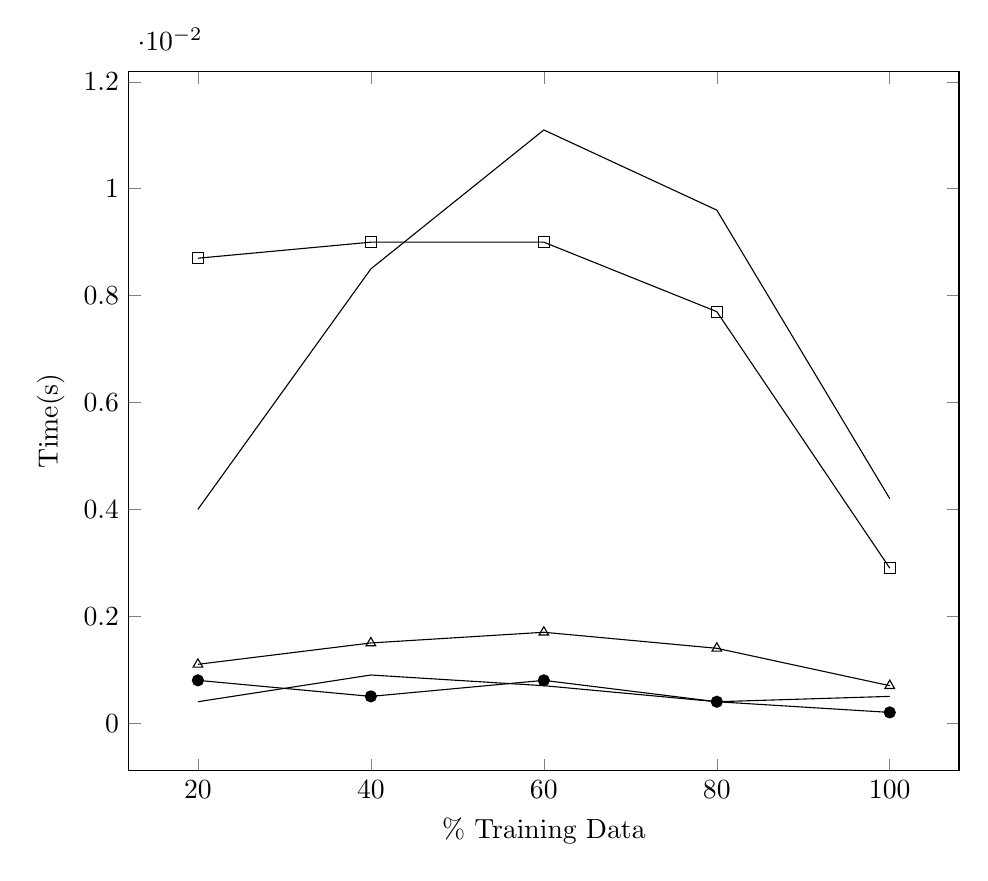
\begin{tikzpicture}
		\begin{axis}[
		width=\textwidth,
		xlabel = \% Training Data,
		ylabel = Time(s),
		xtick=data,
		xticklabels={100,80,60,40,20},
		]
		\addplot[mark=square,error bars/.cd, y dir=both, y explicit, ] coordinates{
			(100,0.0029)
			(80,0.0077)
			(60,0.0090)
			(40,0.0090)
			(20,0.0087)};
		
		\addplot[mark=triangle,error bars/.cd, y dir=both, y explicit, ] coordinates{
			(100,0.0007)
			(80,0.0014)
			(60,0.0017)
			(40,0.0015)
			(20,0.0011)};
		
		\addplot[mark=*,error bars/.cd, y dir=both, y explicit, ] coordinates{
			(100,0.0002)
			(80,0.0004)
			(60,0.0008)
			(40,0.0005)
			(20,0.0008)};
		\addplot[error bars/.cd, y dir=both, y explicit, ] coordinates{
			(100,0.0042)
			(80,0.0096)
			(60,0.0111)
			(40,0.0085)
			(20,0.0040)};
		
		\addplot[error bars/.cd, y dir=both, y explicit, ] coordinates{
			(100,0.0005)
			(80,0.0004)
			(60,0.0007)
			(40,0.0009)
			(20,0.0004)};
		
		
		\end{axis}
		\end{tikzpicture}
	\end{subfigure}
	\caption{Timing Experiment, square = Random Forest, triangle = LMT }
\end{figure} 


\subsection{Supplementary Material}


\section{Conclusions}


\subsection{References}


\bibliographystyle{IEEEtran}
\bibliography{sample_bib.bib}

\end{document}
